\documentclass[tikz,border=2pt]{standalone}
\usepackage{amsmath}
\usepackage{amssymb}
\usepackage{pgfplots}
\pgfplotsset{compat=1.18}
\usetikzlibrary{arrows.meta}
\begin{document}
% Transformation scheme on Example 4.1: each row of min 5x1+3x2, x1+x2<=50, 4x1+3x2=90, x2<=-8, x1>=5, x2 free
% mapped to its standard-form row, arrows labelled with the steps (1-7) that change it; x1=x1'+5, x2=x2^+ - x2^-.
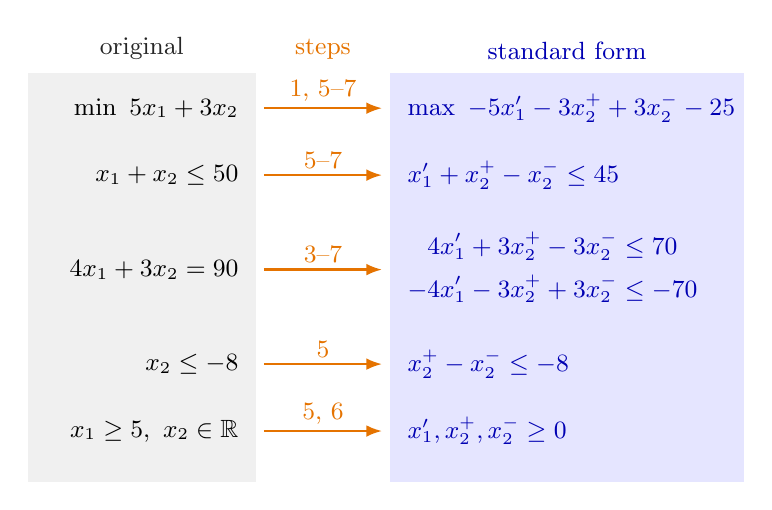
\begin{tikzpicture}[font=\small, >={Latex[length=2mm]}]
  % column backgrounds
  \fill[gray!12] (0,0.45) rectangle (2.9,-4.75);
  \fill[blue!10] (4.6,0.45) rectangle (9.1,-4.75);
  \node[anchor=south, gray!30!black] at (1.45,0.5) {original};
  \node[anchor=south, orange!90!black] at (3.75,0.5) {steps};
  \node[anchor=south, blue!70!black] at (6.85,0.5) {standard form};
  % rows: original -> standard form
  \foreach \y/\orig/\st/\new in {
      0/{$\min\ 5x_1+3x_2$}/{1, 5--7}/{$\max\ -5x_1'-3x_2^{+}+3x_2^{-}-25$},
      -0.85/{$x_1+x_2\leq50$}/{5--7}/{$x_1'+x_2^{+}-x_2^{-}\leq45$},
      -2.05/{$4x_1+3x_2=90$}/{3--7}/{$\begin{aligned}4x_1'+3x_2^{+}-3x_2^{-}&\leq70\\-4x_1'-3x_2^{+}+3x_2^{-}&\leq-70\end{aligned}$},
      -3.25/{$x_2\leq-8$}/{5}/{$x_2^{+}-x_2^{-}\leq-8$},
      -4.1/{$x_1\geq5,\ x_2\in\mathbb{R}$}/{5, 6}/{$x_1',x_2^{+},x_2^{-}\geq0$}} {
    \node[anchor=east] at (2.8,\y) {\orig};
    \draw[orange!90!black, thick, ->] (3.0,\y) -- (4.5,\y) node[midway, anchor=south, inner sep=2pt] {\st};
    \node[anchor=west, blue!70!black] at (4.7,\y) {\new};
  }
\end{tikzpicture}
\end{document}
